
\documentclass{article}
\usepackage[english]{babel}
\usepackage[utf8]{inputenc}
\usepackage{johd}
\usepackage{hyperref}
\usepackage{ulem}
\usepackage{hanging}
 \usepackage{setspace}



    
\title{\textbf{Navigating the Regulatory Framework of Cryptocurrencies: A Fine Balance}}

\author{
        \small \href{https://www.linkedin.com/in/jaidenratti/}{Jaiden Ratti} \\
        \small \href{mailto:jkratti@uwaterloo.com}{jkratti@uwaterloo.ca}\\
        
        \small \newline December 16, 2022
}
\date{}

\doublespace
\begin{document}
\maketitle

\section{Introduction}
\noindent Cryptocurrencies, the leading use-case of blockchain technology, are disrupting traditional financial systems by providing innovative methods of transaction. The decentralized nature of cryptocurrencies, along with the efficiency benefits that come with the removal of intermediaries, is what makes the technology appealing to governments, businesses, and citizens across the globe (Massad, 2019). While the concept of digital currencies has been around for a while, the adoption of cryptocurrencies has seen an exponential increase, with the total market capitalization of all cryptocurrencies surpassing \$1 trillion in 2021 (Hall, 2022). Currently, organizations are recognizing the immense potential of cryptocurrency and the benefits that come with being an early adopter (Tapscott, 2018). Subsequently, as cryptocurrencies play a larger role in the global landscape and impact more people, it is essential for them to be safe, stable, and sustainable.

\noindent \newline To understand the importance and motivations behind maintaining integrity in the cryptocurrency space, it is important to first understand what cryptocurrency is. Cryptocurrencies such as Bitcoin are fully digital coins secured by cryptography that operate on decentralized networks. Users can send these coins in the peer-to-peer network without the need for intermediaries and the high costs normally associated with online transactions. Cryptocurrency transactions are fully traceable and irreversible (Frankenfield, 2022).

\noindent \newline As expected with any innovation, the question of regulation arises. However, the unprecedented rapid growth of cryptocurrency and the inherent function of cryptocurrencies have created special challenges for lawmakers (Cumming et al., 2019). There is stirred debate between the perspectives of pro-regulation for cryptocurrency and anti-regulation for cryptocurrency, and the current diverse regulatory approaches reflect this dichotomy (Global Future Council on Cryptocurrencies, 2021). Government bodies are unsure how to approach the idea of cryptocurrency regulation since they must quickly make policies regarding fairly new technology, meaning policies will have large consequences on future economic prosperity. Countries such as India and China have taken a restrictive regulatory stance, effectively banning the use of cryptocurrency (Global Future Council on Cryptocurrencies, 2021). Whereas countries such as Switzerland and Japan have taken a comprehensive approach, welcoming and regulating cryptocurrency operations by treating them as commodities (Global Future Council on Cryptocurrencies, 2021). There are countless other countries within this spectrum of regulation.

\noindent \newline However, it is evident that the current fragmented cryptocurrency regulatory frameworks create room for regulatory arbitrage resulting in large disparities in innovation and exploitation (Massad, 2019). The aim of this paper is to not only show the importance and need for cryptocurrency regulation but to emphasize the importance of precise and proactive regulation and how to reach this goal to create a safe and productive community for cryptocurrency innovation. The remainder of this paper will achieve this by outlining the need for cryptocurrency regulation in the face of consumer protection, limiting illegal activity, and energy stability, while also refuting common arguments for anti-regulation. The paper will conclude by outlining how different jurisdictions have approached cryptocurrency regulation and taking findings from each of these approaches to ideate new models of regulation to ensure cryptocurrency meaningfully contributes to society.



\section{Motivations for Regulation}
\subsection {The Need for Consumer Protection}

\noindent Cryptocurrencies were designed with the intent to empower the citizens within a society to transact safer, faster, and more efficiently. However, the recent cryptocurrency scandals and frauds have begged the question; what good is a public innovation if it does not have the best interest of the public in mind? Specifically, cryptocurrency exchanges have exposed consumers to unprecedented and immense risk. For reference, cryptocurrency exchanges are platforms that facilitate the buying and selling of cryptocurrencies on a mass scale and allow users to store their cryptocurrency as well (Frankenfield, 2022). However, unlike fiat currency, which is backed by the government, there is no central authority governing these bodies. 

\noindent \newline One of the first demonstrations of this weakness occurred at the cryptocurrency exchange Mt. Gox in 2014. Mt. Gox, known as one of the largest cryptocurrency exchanges at the time, lost over 850,000 bitcoins, worth roughly \$500 million of client money at the time (Ishikawa, 2017). This seismic event was indicated to have happened due to a cyber-attack; however, the real reasons are still unknown (Ishikawa, 2017). In hindsight, Mt. Gox was revealed to have been operating with minimal oversight since there were little to no regulations for cryptocurrency exchanges at the time (Ishikawa, 2017). The exchange had no incentive to install security measures since it would be expensive, and it was not their money at risk. However, after this event, countries such as Japan and the United States introduced regulations for exchanges, requiring them to register with the government and file for licenses (Global Future Council on Cryptocurrencies, 2021).

\noindent \newline In a perfect world, these reactionary regulations enforced by these countries would prevent any future harm. Yet, in late 2022, there is once again a cryptocurrency exchange scam, this time with billions of citizen dollars at stake. One of the largest and most trusted cryptocurrency exchanges, FTX, has recently reported that a significant amount of assets are missing or stolen (Kolhatkar, 2022). In actuality, CEO Sam Bankman-Fried took users’ cryptocurrency deposits and funnelled them to a quantitative trading firm (Kolhatkar, 2022). His goal was to invest consumer deposits as leverage to generate more revenue and this approach was working well (Kolhatkar, 2022). However, in early November of 2022, FTX received an influx of customers wanting to withdraw and sell their cryptocurrencies from the exchange (Kolhatkar, 2022). Unfortunately, FTX did not have enough cryptocurrency on reserve and could not fulfill these requests. FTX had little to no money invested into risk management, proper accounting standards, or ensuring there was enough capital in reserve (Kolhatkar, 2022). It is clear that governments did not learn from the Mt. Gox cryptocurrency attacks, and citizens have paid the price with the collapse of FTX. While the arrest of Sam Bankman-Fried is a symbolic step toward action, policymakers must think hard about regulating exchanges moving forward (Kolhatkar, 2022).

\noindent \newline While in theory, it makes sense to have minimal regulation when it comes to the peer-to-peer nature of cryptocurrency, this theory does not account for bad actors with malicious intent. Implementing regulation for businesses that deal with cryptocurrency will not ruin the integrity of cryptocurrency itself. Ensuring these large corporations are operating in a fair and transparent manner and providing support for users will create confidence in the market, thus increasing adoption.



\subsection{Preventing Illegal Activity in an "Anonymous" Space}

\noindent 
Transacting currency over blockchain technology also arises other complex issues. Using cryptocurrency allows for significantly lower fees, quicker transaction speeds and very importantly, privacy and pseudonymity. This tool creates an opportunity for money laundering, tax evasion and in even extreme cases, financing terrorism. Since transactions do not involve the public release of personal information, addresses, or purpose for sending money, it becomes very enticing to send money for illegal purposes. Looking at the case of the Silk Road marketplace in 2011, cryptocurrency was the backbone of the platform (Metais, 2021). Silk Road was an online digital black marketplace that involved the trading of drugs, stolen credit cards, and even assassinations (Metais, 2021). All transactions were handled in Bitcoin, meaning once the FBI seized the platform, the only person that could be held accountable was the founder of the platform, who is currently serving a life sentence in prison (Metais, 2021). While cryptocurrency transactions are not completely anonymous since transactions can be tracked, it makes it very difficult for law enforcement to trace and prevent funds from being used for illegal activities. Exchanges and platforms using cryptocurrency can be mandated to enact Anti-Money Laundering policies to prevent future Silk Road incidents from happening again.

\noindent \newline This idea of technology being used for illegal activity is not anything new. In the early 2000s, regulators did not remove everyone’s access to the internet once cyberattacks started occurring. Instead, they developed frameworks to make it very hard to create cyber threats. The technology itself is not what is causing the issue, it is the surrounding frameworks in place that dictate interactions and experiences with technology. Proof-of-Work is the proof mechanism used in Bitcoin. It involves “miners” solving complex mathematical problems to validate the transactions and create new transaction blocks. Miners that solve the math problems first are rewarded with cryptocurrency, thus making cryptocurrency mining a very lucrative industry. Companies have invested significant amounts in computer processors and storage facilities to compute these results as fast as possible (Daly, 2022).
\subsection{Energy and Environmental Consequences}

\noindent Thinking holistically, it would be naïve to only analyze cryptocurrency through the lens of its financial and economic impacts. Looking deeper into how cryptocurrencies work, there are immense environmental impacts (OSTP, 2022). Cryptocurrencies can operate because they exist on cryptocurrency algorithms known as consensus mechanisms (Daly, 2022). These consensus mechanisms are what allow different users involved to approve and verify transactions on the network, providing the element of decentralization (Daly, 2022). This process of approving transactions is referred to as “mining” in the cryptocurrency space. The main consensus mechanism used by cryptocurrencies is Proof-of-Work (PoW) (Daly, 2022).

\noindent \newline However, what many tend to not realize is that this computing power uses a substantially large amount of energy (OSTP, 2022). The electricity used to maintain all cryptocurrency transactions in 2022 was approximately 180 billion kilowatt-hours, larger than the national consumption of most third and second-world countries (OSTP, 2022). For reference as to how large this number is, see Appendix A (OSTP, 2022). The amount of electricity consumed and thus greenhouse gases produced is an oversight when thinking in the short-term but is a vital element to keep under control in the long term. If not regulated, cryptocurrencies could continue to create more environmental damage, leaving nobody accountable. Not to mention, the increased popularity of cryptocurrency mining is also creating shortages in the technology industry, resulting in higher electricity bills, skewed demand, and product shortages (OSTP, 2022). There are currently no incentive structures for cryptocurrencies to reduce this negative externality and it is currently seen as a ‘necessary evil’.

\section{Anti-Regulation Concerns and Refutations}
\subsection{``Regulation will Stifle Innovation"}

\noindent While these are pressing arguments for regulation and digital governance, proponents in the cryptocurrency industry also have anti-regulation arguments. The first main argument is that government regulation will stifle innovation (Newbery, 2021). However, this argument is largely a straw man argument, misrepresenting the idea of regulation. While there is a chance of this happening depending on the appropriate government, this is a worst-case scenario. If anything, regulation can advance innovation by setting a foundation of rules and guidelines for companies to follow (Werbach, 2021). If businesses have a steady and clearly define environment to operate in, then that will reduce friction to innovate and even increase innovation. However, it is important to note that these conditions are contingent on the regulatory frameworks in place.

\subsection{``Regulation Goes Against Decentralization"}
\noindent Another main point for anti-regulation is the perpetuated idea that the function of cryptocurrencies is to be decentralized and excluded from government control, thus there should be no regulation (Newbery, 2021). While it is true that cryptocurrencies are meant to be decentralized, this does not automatically omit them from government control. Since citizens and businesses within a society are using cryptocurrency, the government has the responsibility to financially protect consumers within the economy. This idea of appealing to tradition and not imposing regulation since regulation did not exist when cryptocurrency was first created is short-sighted (McDonald, 2021). Governments should still be able to regulate the businesses that operate within their borders and not exempt them from laws since they operate with cryptocurrency instead of fiat currency. Governments must protect their citizens from corporations with malicious intent regardless of transaction methods.


\section{Regulatory Frameworks for Cryptocurrency}
\subsection{The Current Fragmented State of Regulation}

\noindent The premise of anti-regulation is important to think about in the process of regulation when finding common ground. Countries across the world have taken varying stances on regulating cryptocurrencies, with some approaches being more effective than others. The big question these governing bodies set out to answer is how they can regulate the industry to protect consumers now and in the future without hurting innovation.

\noindent \newline Brazil has adopted a ‘wait and see’ approach, enforcing no specific regulations for cryptocurrencies (Global Future Council on Cryptocurrencies, 2021). Instead, they are letting cryptocurrency grow under the normal frameworks of the financial sector. This approach has significantly increased cryptocurrency innovation, however, requires very active policymakers and exposes citizens to risk (Global Future Council on Cryptocurrencies, 2021). On the same spectrum, the U.A.E has a specific set of regulations for cryptocurrencies created by the Central Bank of the United Arab Emirates and the Securities and Commodities Authority (Global Future Council on Cryptocurrencies, 2021). This approach has resulted in U.A.E becoming a global hotspot for cryptocurrency innovation. U.A.E believes that the risk of over-regulation is more appealing than the risk of under-regulation. Countries such as China and India have banned any sort of crypto- related business within their country (Global Future Council on Cryptocurrencies, 2021). These actions are reflective of their political systems and ideologies. The United States has taken an approach that mainly consists of categorizing different elements of cryptocurrency into pre- existing asset classes and thus governing accordingly (Massad, 2019). The Securities and Exchange Commission, as well as the Commodity Futures Trading Commission, are both responsible for regulating different aspects, however, this regulation remains unclear (Massad, 2019). This approach of trying to fit a square peg into a round hole has not reaped great results for the country.

\subsection{Looking Ahead to the Future of Ideal Regulation}

\noindent A fundamental aspect of creating effective regulatory policies is taking a multistakeholder approach. This will reduce the regulatory burden that the government currently faces. There is currently a disconnect between cryptocurrency businesses and lawmakers, creating an ‘us versus them’ mentality (Tapscott, 2018). Strong regulation requires collaboration and compromise between the public sector and the private sector. The private sector understands the capabilities of the technology and the demand, and the public sector can use this information to create regulatory frameworks (Tapscott, 2018). However, it is first important to be decisive in terms of defining the asset class of cryptocurrency and setting clear guidelines. Then, there should be uniform regulation across jurisdictions. Imposing cryptocurrency exchange regulation should also be a priority. Setting capital reserve requirements and requiring licenses should be the starting point of exchange regulation. Overall, the peer-to-peer underpinning of cryptocurrency is difficult to regulate within borders since the idea is borderless (Cumming et al., 2019). 

\noindent \newline Collaboration and distributing the regulatory burden among the network and taking inspiration from the decentralized nature of cryptocurrency can be effective ways of creating cryptocurrency policies that protect consumers.


\section{Concluding Thoughts}

\noindent Navigating the fine line of cryptocurrency regulation is a complicated and contentious matter for governments across the globe. It is important that governments understand the impact of cryptocurrencies, both positive and negative, and act accordingly. While regulation can never be perfect, some form of precise regulation is essential in preserving the disruptive elements of cryptocurrency. In the facets of cryptocurrency regulation, policymakers must keep consumer protection, preventing illegal activity, and energy conservation at the forefront of decisions. Countries have a lot to learn from each other in terms of giving cryptocurrency the opportunity to create the economic prosperity and financial inclusivity it was intended to enable. Future research into cases of cryptocurrency companies collaborating with governments can help provide further insight into the direction of cryptocurrency regulation and the necessary steps to take.


\newpage \title\noindent\textbf{References}
\begin{hangparas}{.25in}{1}

Cumming, D. J., Johan, S., \& Pant, A. (2019). Regulation of the Crypto-Economy: Managing Risks, Challenges, and Regulatory Uncertainty. Journal of Risk and Financial Management, 12(3), 126. \url{http://dx.doi.org/10.3390/jrfm12030126}.\\

Daly, L. (2022, June 28). What is Proof of Work (PoW) in crypto? The Motley Fool. \url{https://www.fool.com/investing/stock-market/market-sectors/financials/cryptocurrency- stocks/proof-of-work/}\\

\newline Frankenfield, J. (2022, September 26). Cryptocurrency explained with pros and cons for investment. Investopedia. \url{https://www.investopedia.com/terms/c/cryptocurrency.asp}\\

\newline Global Future Council on Cryptocurrencies. (2021). Navigating cryptocurrency regulation: An industry perspective on the insights and tools needed to shape balanced crypto regulation. World Economic Forum. \url{https://www3.weforum.org/docs/WEF_Navigating_Cryptocurrency_Regulation_2021.pdf}\\

\newline Hall, J. (2022, July 18). Crypto recaptures \$1 trillion market cap: BTC this \$22k, ETH ‘Giga mooning’. Cointelegraph. \url{https://cointelegraph.com/news/crypto-recaptures-1-trillion- market-cap-btc-hits-22k-eth-giga-mooning}\\

\newline Ishikawa, M. (2017). Designing virtual currency regulation in Japan: Lessons from the Mt Gox case. Journal of Financial Regulation, Volume 3, Issue 1, 125-131. \url{https://doi.org/10.1093/jfr/fjw015}\\

\newline Kolhatkar, S. (2022, November 23). Will the FTX collapse lead to better cryptocurrency regulation. The New Yorker. \url{https://www.newyorker.com/business/currency/will-the-ftx- collapse-lead-to-better-cryptocurrency-regulation}\\

\newline Massad, T. G. (2019, March). It’s time to strengthen the regulation of crypto-assets. Economic Studies at Brookings. \url{https://www.brookings.edu/wp- content/uploads/2019/03/Economis-Studies-Timothy-Massad-Cryptocurrency-Paper.pdf}\\

\newline McDonald, O. (2021). Cryptocurrencies: Money, Trust and Regulation. Columbia University Press. \url{http://cup.columbia.edu/book/cryptocurrencies/9781788214209}\\

\newline Metais, J. (2021, August 20). Silk Road. CoinDesk. \url{https://www.coindesk.com/company/silk- road}/\\

\newlineNewbery, E. (2021, October 21). Do we need more crypto regulation? Two sides of the story. Motley Fool. \url{https://www.fool.com/the-ascent/cryptocurrency/articles/do-we-need-more- crypto-regulation-two-sides-of-the-story/}\\

\newline OSTP. (2022). Climate and Energy Implications of Crypto-Assets in the United States. White House Office of Science and Technology Policy. \url{https://www.whitehouse.gov/wp- content/uploads/2022/09/09-2022-Crypto-Assets-and-Climate-Report.pdf}\\

\newline Tapscott, D. (2018, August). 2018 Blockchain regulation roundtable: Addressing the regulatory challenges of disruptive innovation. Blockchain Research Institute. \url{https://www.blockchainresearchinstitute.org/project/2018-regulation-roundtable/}\\

\newline Werbach, K. (2021, April 27). Why regulation won’t harm cryptocurrencies. Knowledge at Wharton. \url{https://knowledge.wharton.upenn.edu/article/why-regulation-wont-harm- cryptocurrencies/}\\

\end{hangparas}


\newpage \title\centering{\textbf{Appendix}}
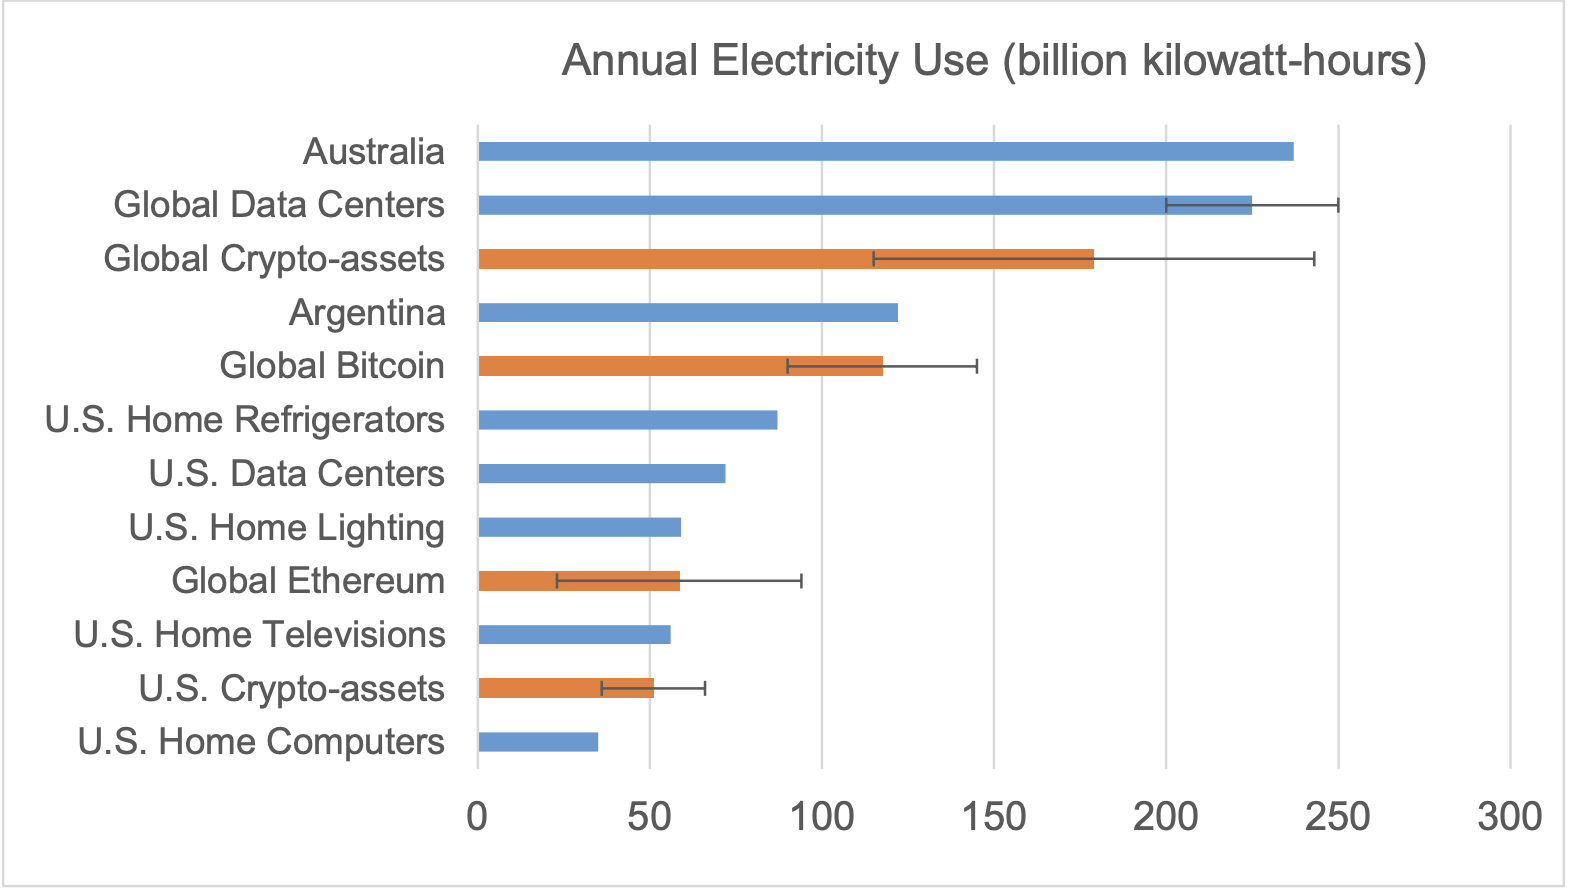
\includegraphics[width=\textwidth]{electricity.png}

\noindent \newline Figure A1. This graph compares various annual electricity usage in billion kilowatt-hours and estimates for crypto assets as of August 2022. The error bars are included to provide a more accurate range of values.


\end{document}
